\documentclass{article}
\usepackage{amssymb,amsmath}
\usepackage{ifxetex,ifluatex}
\ifxetex
  \usepackage{fontspec,xltxtra,xunicode}
  \defaultfontfeatures{Mapping=tex-text,Scale=MatchLowercase}
\else
  \ifluatex
    \usepackage{fontspec}
    \defaultfontfeatures{Mapping=tex-text,Scale=MatchLowercase}
  \else
    \usepackage[utf8]{inputenc}
  \fi
\fi
\usepackage{ctable}
\usepackage{float} % provides the H option for float placement
\usepackage{graphicx}
% We will generate all images so they have a width \maxwidth. This means
% that they will get their normal width if they fit onto the page, but
% are scaled down if they would overflow the margins.
\makeatletter
\def\maxwidth{\ifdim\Gin@nat@width>\linewidth\linewidth
\else\Gin@nat@width\fi}
\makeatother
\let\Oldincludegraphics\includegraphics
\renewcommand{\includegraphics}[1]{\Oldincludegraphics[width=\maxwidth]{#1}}
\ifxetex
  \usepackage[setpagesize=false, % page size defined by xetex
              unicode=false, % unicode breaks when used with xetex
              xetex]{hyperref}
\else
  \usepackage[unicode=true]{hyperref}
\fi
\hypersetup{breaklinks=true, pdfborder={0 0 0}}
\setlength{\parindent}{0pt}
\setlength{\parskip}{6pt plus 2pt minus 1pt}
\setlength{\emergencystretch}{3em}  % prevent overfull lines
\setcounter{secnumdepth}{0}

\title{Outlier test}
\author{Rapport package team @ https://github.com/aL3xa/rapport}
\date{2011--04--26 20:25 CET}

\begin{document}
\maketitle

\subsection{Description}

This template will check if provided variable has any outliers.

\subsubsection{Boxplot}

\begin{figure}[htbp]
\centering
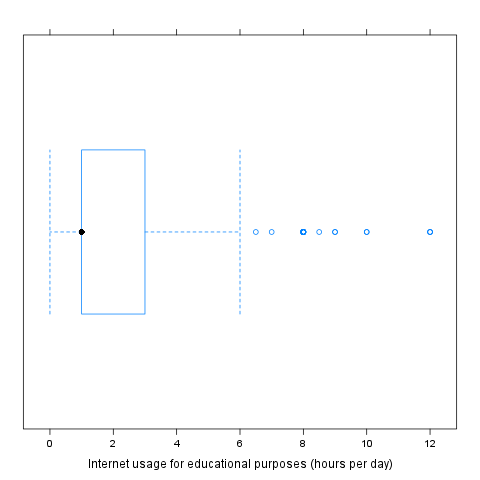
\includegraphics{d30dda4b6d42b184f75e9550cae167eb.png}
\caption{}
\end{figure}

\subsubsection{Lund test}

It seems that 5 extreme values can be found in ``Internet usage for
educational purposes (hours per day)''. These are: 10, 10, 12, 12, 12.

\paragraph{Explanation}

The above test for outliers was based on \emph{lm(1 \ensuremath{\sim}
it.edu)}:

\ctable[pos = H, center, botcap]{lllll}
{% notes
}
{% rows
\FL
 & \textbf{Estimate} & \textbf{Std. Error} & \textbf{t
value} & \textbf{Pr(\textgreater{}\textbar{}t\textbar{})}
\ML
(Intercept) & 2.06276 & 0.07663 & 26.91942 & 0.00000
\LL
}

\paragraph{The residuals returned:}

\ctable[pos = H, center, botcap]{l}
{% notes
}
{% rows
\FL
--0.03078, 2.91195, --0.27601, --0.52124, --0.52124, --0.76647,
--1.01169, --0.27601, --0.52124, 1.44058, --0.52124, 0.95013, 3.89286,
--0.03078, --0.52124, --0.76647, --0.03078, 1.44058, --0.52124, 0.45967,
1.93104, --0.52124, 0.95013, --0.52124, 0.95013, --0.03078, 0.45967,
--0.76647, 0.95013, --0.76647, --0.52124, --0.52124, --0.52124, 1.44058,
3.40240, --0.52124, --0.52124, --0.27601, --0.52124, --0.52124,
--0.76647, --0.76647, 0.95013, 0.45967, --0.52124, 1.44058, 1.44058,
--0.52124, --0.76647, 0.45967, --0.03078, 1.44058, --0.52124, 2.91195,
0.45967, --0.76647, 1.44058, 0.95013, 1.44058, --0.76647, --0.52124,
--0.03078, --0.76647, --0.52124, 0.45967, --0.76647, 0.95013, --0.76647,
--0.52124, --0.76647, --0.03078, --0.52124, 0.45967, 0.45967, --0.03078,
--0.76647, --1.01169, --0.76647, --0.52124, --0.52124, --0.27601,
--0.76647, --0.76647, 2.91195, --0.03078, 2.91195, 0.45967, --0.03078,
--0.52124, --0.52124, --0.27601, --0.76647, 0.95013, --0.52124,
--0.03078, --0.76647, 0.70490, --0.52124, --0.76647, --0.52124, 0.21444,
--0.03078, --0.03078, --0.03078, --1.01169, --0.76647, --0.27601,
2.91195, --1.01169, 1.19535, 0.95013, 2.91195, --0.27601, --0.03078,
0.95013, --0.76647, --1.01169, --0.76647, --0.52124, 0.45967, --0.76647,
--1.01169, 2.91195, --0.52124, --0.76647, --0.52124, --0.76647,
--0.52124, --1.01169, --0.52124, 2.42149, --0.52124, --0.52124, 1.44058,
0.21444, 0.21444, 0.95013, 0.45967, 0.21444, --0.27601, 0.95013,
1.93104, --0.76647, 0.21444, --0.03078, --0.52124, --1.01169, --1.01169,
--0.03078, --0.03078, --0.03078, --0.76647, --0.52124, --0.52124,
--0.52124, --0.52124, --0.52124, --1.01169, --0.52124, 0.45967,
--0.03078, --0.52124, 0.45967, --0.76647, 0.21444, 1.44058, 1.44058,
--1.01169, 1.44058, 0.95013, --0.76647, --0.52124, --0.76647, --0.76647,
--0.03078, --0.52124, 0.45967, --0.03078, --0.52124, --0.52124,
--0.03078, --0.76647, --0.52124, 2.91195, --0.76647, --0.76647,
--0.52124, --0.76647, --0.03078, --0.03078, --0.76647, --0.52124,
--0.52124, --1.01169, --0.52124, --0.52124, 0.45967, --0.03078, 0.45967,
--0.52124, --0.52124, --1.01169, --1.01169, --0.03078, --1.01169,
--0.52124, --0.52124, 0.95013, --0.76647, 2.91195, --0.52124, --0.03078,
--1.01169, 1.44058, 0.45967, --0.52124, --0.03078, --0.76647, --0.52124,
--0.52124, --1.01169, --0.76647, --0.76647, --1.01169, --0.76647,
--0.52124, 0.45967, --0.03078, --0.03078, --1.01169, --0.76647,
--0.52124, --0.03078, --0.52124, --0.03078, --1.01169, 0.95013, 0.45967,
--0.03078, --0.03078, 0.45967, --0.52124, --1.01169, 2.91195, --0.03078,
--0.52124, 0.95013, --0.52124, --0.03078, 3.40240, 0.45967, --0.52124,
--0.52124, --0.52124, --0.03078, --0.76647, --0.52124, --0.76647,
--0.76647, --0.52124, --1.01169, --0.52124, 0.45967, --0.03078,
--0.52124, --0.03078, --0.52124, --0.52124, 0.45967, --1.01169,
--0.03078, --0.76647, 3.89286, 0.45967, --0.76647, 0.45967, --1.01169,
--0.76647, --0.76647, --0.03078, --0.27601, --0.03078, --0.76647,
--0.76647, --0.03078, 0.45967, --0.52124, --0.52124, --0.52124,
--0.03078, --0.27601, --0.52124, --0.03078, 1.93104, 1.93104, 2.91195,
--0.76647, 0.45967, 4.87377, --0.76647, 1.44058, 2.91195, --0.52124,
0.95013, --1.01169, --0.52124, 2.91195, --0.03078, 2.91195, --0.52124,
0.95013, 0.95013, 0.45967, --0.52124, --0.27601, --0.52124, --0.76647,
--0.52124, --0.52124, --0.52124, --0.52124, 0.45967, --0.76647, 1.44058,
--0.52124, --0.03078, --0.03078, --0.03078, --0.52124, --0.52124,
--0.76647, 1.93104, --0.52124, --0.03078, --0.52124, --1.01169,
--0.52124, 0.45967, --0.76647, --0.52124, 0.45967, --0.52124, 4.87377,
--0.52124, --0.27601, --0.52124, 0.45967, --1.01169, --0.76647,
--0.52124, 2.91195, 1.44058, --0.03078, --0.27601, 1.93104, 2.91195,
--0.52124, 2.91195, 0.45967, --0.52124, 0.95013, 0.21444, --0.03078,
--0.52124, --1.01169, --1.01169, 1.68581, 0.21444, --0.52124, --0.52124,
--0.27601, --1.01169, --0.52124, --1.01169, --0.52124, --0.76647,
--0.52124, 0.45967, --0.03078, --1.01169, --0.03078, 0.45967, 0.45967,
0.45967, --0.52124, --0.52124, 2.91195, --0.52124, --1.01169, 2.91195,
--1.01169, --0.52124, 0.45967, --1.01169, 1.44058, --0.03078, 0.95013,
--1.01169, 2.91195, --0.52124, --0.76647, 0.95013, --0.03078, --0.52124,
0.21444, --0.03078, --0.52124, --0.76647, 4.87377, 1.93104, 0.95013,
--0.03078, 0.95013, 1.19535, 0.45967, --0.76647, --0.76647, --1.01169,
0.95013, 2.91195, 0.45967, 1.44058, 2.91195, --0.52124, 0.45967,
1.44058, --1.01169, --0.03078, 0.45967, --0.03078, 1.93104, --0.52124,
--0.52124, 1.44058, --0.03078, --0.52124, --0.76647, --0.52124,
--0.52124, 0.21444, --0.52124, --0.52124, --0.52124, --0.52124,
--0.03078, --0.76647, --0.03078, 0.95013, --0.52124, 0.45967, --0.03078,
--0.76647, --0.03078, --0.52124, --0.52124, --0.52124, --0.03078,
--0.52124, --0.52124, --0.76647, --0.52124, --0.27601, --0.76647,
--0.03078, --0.76647, --0.52124, 1.44058, --1.01169, 0.95013, --0.03078,
--0.76647, --0.76647, --0.52124, --0.52124, --0.52124, --0.52124,
--0.03078, --0.76647, --0.52124, --0.52124, --0.52124, --0.52124,
0.70490, --0.03078, --0.52124, 0.45967, --0.03078, --0.52124, --0.76647,
--0.52124, --0.76647, --1.01169, --0.03078, --0.52124, --0.03078,
0.95013, --0.52124, --0.52124, --0.03078, --0.76647, --0.52124, 0.21444,
--0.27601, --0.03078, --0.52124, --0.76647, --0.52124, --0.03078,
--0.03078, --0.52124, --0.03078, --0.52124, 1.93104, --0.27601, 1.93104,
--0.52124, --0.52124, --0.27601, --0.52124, --0.03078, 0.45967,
--0.76647, --0.52124, 0.45967, 0.95013, --0.03078, 1.44058, --0.52124,
0.45967, 0.45967, --0.52124, --0.27601, 0.21444, 1.44058, --0.27601,
1.44058, --0.03078, 0.45967, 1.44058, --0.52124, --0.27601, --0.52124,
--0.52124, --0.03078, --0.52124, --0.03078, --0.76647, --0.76647,
--0.76647, --0.52124, --0.76647, --0.52124, --0.27601, --0.03078,
0.45967, 0.95013, --1.01169, --0.27601, 1.93104, 1.93104, --0.52124,
--0.52124, 0.45967, --0.52124, 0.95013, --0.52124, --1.01169, --0.03078,
0.95013, --0.76647, --0.03078, 0.95013, --0.52124, --0.27601, 2.17627,
--0.03078, 0.95013, 0.45967, 1.44058, 0.21444, --0.76647, --0.52124,
--1.01169, --0.03078, 0.45967, --0.76647, --1.01169, --1.01169,
--0.52124, --0.52124, --0.03078, --0.52124, --0.27601, --1.01169,
--0.03078, 0.45967, --0.76647, --0.52124, --0.52124, --0.52124,
--0.03078, --0.52124, --0.52124, 0.45967, --0.52124, --1.01169,
--1.01169, 0.45967, --0.27601, --0.52124, 1.93104, --0.03078, --0.52124,
--1.01169, --0.52124, --0.76647, --1.01169, 0.95013, 0.95013, 1.44058,
--0.76647, --0.52124, --0.52124, --0.03078, 1.44058, --1.01169, 0.45967,
--0.52124, 1.44058, 0.45967, --0.76647, --0.52124, --0.76647, --1.01169,
--0.76647, --0.76647, --0.03078, --1.01169, 0.21444, 0.45967, 2.91195,
0.45967, --0.76647, --0.76647, --0.03078, 0.21444, --0.03078, 0.45967,
--0.52124, 0.21444, 2.91195, --1.01169, --0.52124, --0.52124, 1.44058,
--0.52124, --0.27601, --1.01169, --0.03078, --0.03078, --0.03078,
0.21444, --1.01169, 0.45967, --0.52124, --0.76647, --0.52124, --0.76647,
--0.03078, --0.52124, 0.45967, --0.52124, --1.01169, --0.03078,
--0.03078, --0.03078, --0.03078, 1.44058, 0.95013, --1.01169, --0.03078,
1.44058, --0.52124, --0.03078, 0.45967, --0.52124, 1.44058, 0.45967,
--0.52124, 0.45967, --0.52124, --0.76647, --0.52124, --1.01169,
--0.76647, --0.03078, --0.52124, --0.76647, --0.03078, --0.76647,
--0.52124, --0.52124, --0.76647, 2.91195, 3.15718, --1.01169, --1.01169,
--0.76647, --0.52124
\LL
}

\paragraph{References}

\ctable[pos = H, center, botcap]{l}
{% notes
}
{% rows
\FL
* Lund, R. E. 1975, ``Tables for An Approximate Test for Outliers in
Linear Models'', Technometrics, vol.~17, no. 4, pp.~473--476.
\\\noalign{\medskip}
* Prescott, P. 1975, ``An Approximate Test for Outliers in Linear
Models'', Technometrics, vol.~17, no. 1, pp.~129--132.
\LL
}

\subsubsection{Grubb's test}

\ctable[pos = H, center, botcap]{l}
{% notes
}
{% rows
\FL
Grubbs test for one outlier shows that highest value 12 is an outlier
(p=0.00032).
\LL
}

\paragraph{References}

\ctable[pos = H, center, botcap]{l}
{% notes
}
{% rows
\FL
* Grubbs, F.E. (1950). Sample Criteria for testing outlying
observations. Ann. Math. Stat. 21, 1, 27--58.
\LL
}

\subsubsection{Dixon's test}

\ctable[pos = H, center, botcap]{l}
{% notes
}
{% rows
\FL
chi-squared test for outlier shows that highest value 12 is an outlier
(p=0).
\LL
}

\paragraph{References}

\ctable[pos = H, center, botcap]{l}
{% notes
}
{% rows
\FL
* Dixon, W.J. (1950). Analysis of extreme values. Ann. Math. Stat. 21,
4, 488--506.
\LL
}

\end{document}
